

\usetikzlibrary{shapes.geometric} 
\pgfdeclareplotmark{mystar}{
    \node[star,star point ratio=2.25,minimum size=6pt,
          inner sep=0pt,draw=black,solid,fill=red] {};
}
\definecolor{tiffanyblue}{RGB}{129,216,208}
\definecolor{bangdiblue}{RGB}{0,149,182}
\definecolor{kleinblue}{RGB}{0,47,167}
\definecolor{kabuliblue}{RGB}{26,85,153}
\definecolor{purple}{RGB}{138,43,226}
\definecolor{upink}{RGB}{255,150,128}
\begin{figure}[t!]
\centering
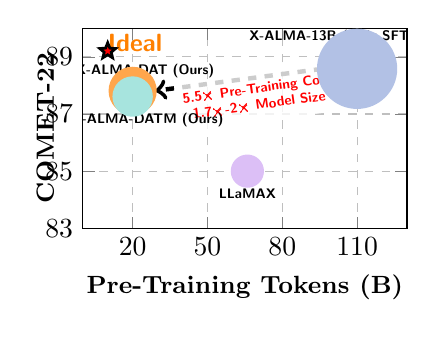
\begin{tikzpicture}
  \pgfplotsset{set layers}
      \begin{axis}[
	 at={(0,0)},
      ymajorgrids,
      xmajorgrids,
      grid style=dashed,
      width=0.47*\textwidth,
      height=0.34*\textwidth,
      legend style={at={(0.23,0.08)}, anchor=south west},
      xlabel={\small{Pre-Training Tokens (B)}},
      ylabel={\small{COMET-22}},
      ylabel style={font=\bfseries,yshift=-1em, xshift=0em},xlabel style={font=\bfseries,xshift=0em,yshift=0.0em},
      yticklabel style={/pgf/number format/precision=0,/pgf/number format/fixed zerofill},
      ymin=83,ymax=90, ytick={83, 85, 87, 89},
      xmin=0,xmax=130,xtick={20, 50, 80, 110},
      legend style={yshift=-6pt,xshift=-2em, legend plot pos=right,font={\footnotesize},cells={anchor=west}}
      ]
    \addplot[kleinblue!30,mark=*,mark size=14pt,thick,mark options={fill=kleinblue!30,draw=kleinblue!30,line width=1.0pt}] coordinates { (110,88.58)
    };
    \node at (axis cs:100,89.7) [font=\bfseries\sffamily\tiny] {X-ALMA-13B (Only SFT)};
      
      
    \addplot[orange!70,mark=*,mark size=8.2pt,thick,mark options={fill=orange!70, draw=orange!70,line width=1.0pt}] coordinates { (20,87.81)
    };
    \node at (axis cs:25,88.5) [font=\bfseries\sffamily\tiny] {X-ALMA-DAT (Ours)};

    \addplot[tiffanyblue!70,mark=*,mark size=6.8pt,thick,mark options={fill=tiffanyblue!70, draw=tiffanyblue!70,line width=1.0pt}] coordinates { (20,87.61)
      };
      
    \addplot[purple!30,mark=*,mark size=5.5pt,thick,mark options={fill=purple!30,line width=1.0pt}] coordinates { (66,85.00)
      };
    \node at (axis cs:66,84.2) [font=\bfseries\sffamily\tiny] {LLaMAX};

    \addplot[only marks,red!50,mark=mystar,mark size=5pt,thick,mark options={fill=red!50, draw=red!50,line width=1.0pt}, scale=2] coordinates {(10, 89.2)
    };
    \node at (axis cs:21,89.50) [orange, font=\bfseries\sffamily\small] {Ideal};

    \draw[dashed, ->, ultra thick] 
    (axis cs:96, 88.58) -- (axis cs:29, 87.81);

    \node[red, align=center, font=\bfseries\sffamily\tiny, fill=white, opacity=0.8, text opacity=1, rounded corners, rotate=8] 
   at (axis cs:73, 87.6) 
   {5.5× Pre-Training Cost ↓ \\ 1.7×-2× Model Size ↓};
   \node at (axis cs:26,86.8) [font=\bfseries\sffamily\tiny] {X-ALMA-DATM (Ours)};
    
      \end{axis}

      
  \end{tikzpicture}
\vskip -0.1in
    \caption{The relationship between pre-training cost, model capacity and translation performance. We evaluate performance on the Flores-200 test sets across 50 languages. \textbf{The size of circle denotes model capacity.}}
    \label{fig:curse_of_multilinguality}
\end{figure}
